%!TEX root = thesis.tex

% ~10 pages 

\chapter{Conceptual system architecture}
\label{chap:design}

This thesis aims to design a conceptual system architecture that uses the semantic web to improve sensor data discovery as well as the integration and aggregation of sensor data from multiple sources. The outline of this architecture will be described here using the methods of Chapter \ref{chap:methods}. 

\section{Creating linked data from sensor metadata}
\label{par:Architecture1}
The proposed process of automatically creating linked data from sensor metadata is shown in Figure \ref{fig:WPS1}. A \acf{wps} should be created containing processes for retrieving metadata, converting it to linked data and outputting it to a triple store. The data of a \ac{sos} is retrieved by a \ac{wps} process and automatically converted to linked data. The output are \ac{rdf} documents containing the metadata as triples. These documents are posted to a \ac{sparql} endpoint, where they can be queried using \ac{sparql}.  

The workflow of this \ac{wps} process is shown in Figure \ref{fig:WPS1workflow}. It is an adaption of the workflow by \cite{LD:Missier}, which was originally intended for creating linked data of vector parcel data. The input of the process is the \ac{http} address of a \ac{sos}. Since both the requests and the data model are standardised in a \ac{sos}, the process should be able to automatically perform the tasks for creating linked data. The first step is to make requests to the \ac{sos} to retrieve its metadata. This results in a number of \ac{xml} documents that need to be filtered. The second step is to map the data inside these \ac{xml} documents to linked data ontologies. In the final step \ac{rdf} documents are created of the mapped metadata and published on the web.  

\begin{figure}
	\centering
	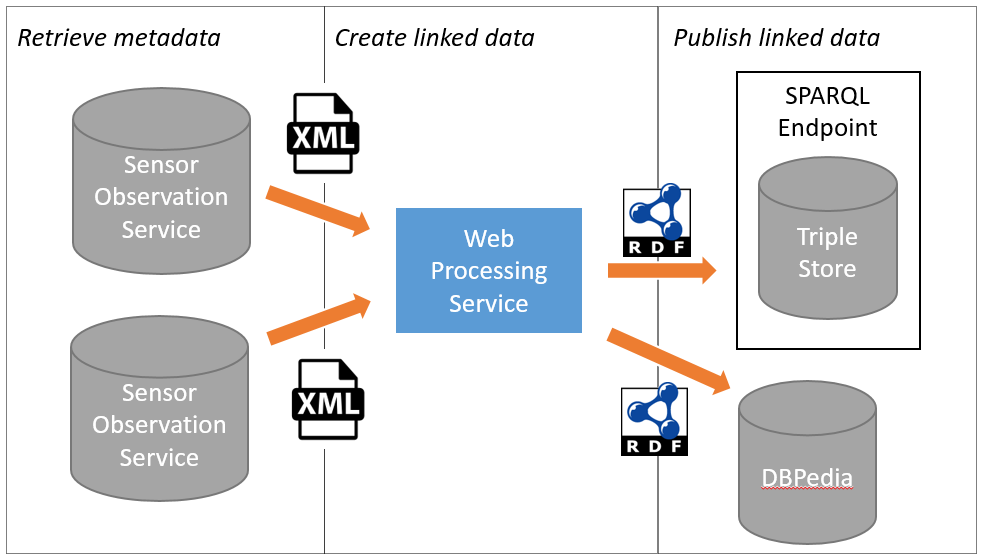
\includegraphics[width=0.8\linewidth]{UML/wps1diagram2.PNG}
	\caption{General overview of creating linked data of metadata from Sensor Observation Services}
	\label{fig:WPS1}
\end{figure}

\begin{figure}
	\centering
	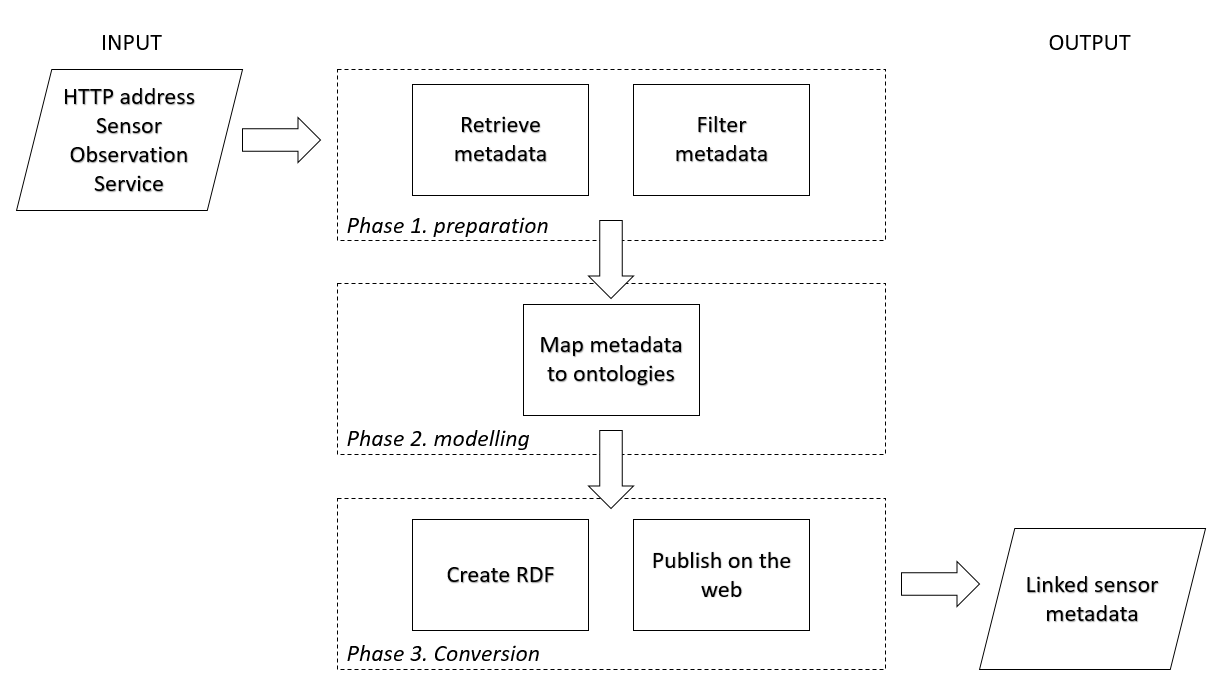
\includegraphics[width=1\linewidth]{UML/wps1workflow.PNG}
	\caption{Workflow diagram of web process for creating linked sensor metadata (adapted from \cite{LD:Missier})}
	\label{fig:WPS1workflow}
\end{figure}

\subsection{Retrieving metadata from the Sensor Observation Service}
\label{chap:retrieveSOS}

The first step of creating an online knowledge base with sensor metadata is to retrieve the metadata from the different \aclp{sos}. This data has to be understood in order to map it to an ontology and it should be filtered to only contain the required parts of data. The following will describe the way sensor metadata is modelled in a \ac{sos} (Figure \ref{fig:SOS_UML}), with which requests it can be retrieved and how it should be filtered. 

\subsubsection{Sensor metadata model}
In the capabilities document a \ac{sos} describes a number of its properties, providing an overview of its metadata for clients looking for observation data. It identifies the organisation that maintains it, with at least the organisation's name and its contact information. Optionally, the organisation's website, keywords and an abstract about the \ac{sos} can be supplied. The \ac{sos} also describes its identifier and its \ac{http} addresses for sending POST or GET requests. It also lists the \ac{sos} versions and response formats it supports. The access constraints and fees are also mentioned. In most cases the use is free of charge and without access constraints. However, it is possible for an organisation to restrict the use of the \ac{sos} in these ways.  

In the \ac{swe} standards a sensor is modelled using two entities: a procedure and a \acf{foi}. The procedure is the method of sensing and the \ac{foi} is the feature (sampling point) of which a certain property is being sensed. Roughly speaking, the \ac{foi} holds the sensor's location when it made an observation and the procedure describes the type of sensor. Therefore, the observable property ties together the procedure and feature of interest (Figure \ref{fig:SOS_UML}). It should be noted that on an abstract level the \ac{foi} does not necessarily have to be represented by a point geometry. It can also be generalized into larger features (e.g. multiple sensors observing different parts of a lake, where the lake is the ultimate \ac{foi}). 

In version 2.0 of the \acl{sos} Interface Standard \citep{SW:OGC2} an offering is defined as a grouping of \acp{foi}, which have a common procedure. The constraint of sharing the same procedure has been added in version 2 of this document, to solve the ambiguity of offerings in \ac{sos} 1.0. The purpose of offerings is to allow users to query the observation data more efficiently. \acp{foi} that are often queried together are therefore grouped into the same offering for efficient retrieval.        

\begin{figure}
	\centering
	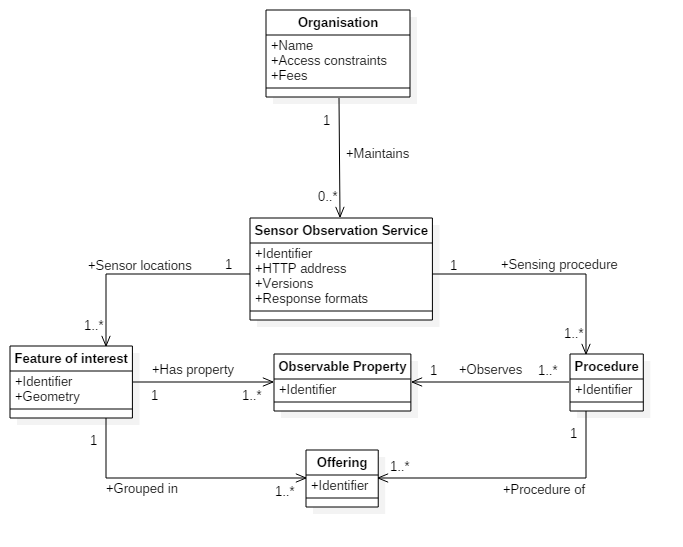
\includegraphics[width=\linewidth]{UML/SOS_UML.PNG}
	\caption{Sensor metadata retrieved from a \ac{sos}}
	\label{fig:SOS_UML}
\end{figure}

\subsubsection{Metadata Requests}
\label{par:metadataRequests}
To retrieve metadata from a \ac{sos} a \texttt{GetCapabilities} request is made first. This is a request with a very generic structure. The GET request is created by adding \url{service=SOS\&request=GetCapabilities} to the \ac{http} address of the \ac{sos}. For example, the \ac{rivm} has its \ac{sos} at the address: \url{http://inspire.rivm.nl/sos/eaq/service?}. Therefore, the capabilities document can be retrieved using the following \ac{url}: \url{http://inspire.rivm.nl/sos/eaq/service?service=SOS&request=GetCapabilities}. 

This requests returns the capabilities document of the \ac{sos} (see Subsection \ref{par:capabilities}). This lists the identifier of each \ac{foi}, each procedure and each observed property. It also has a section where the offerings that it contains are being described. This description of an offering includes a unique identifier, a procedure and the corresponding observed property. Additionally, descriptions can be added such as a bounding box, temporal range, \ac{foi} type and response format.  

\begin{sloppypar}
	The capabilities document is unfortunately not able to provide information about which procedure is being applied for which feature of interest. This is crucial information for knowing which deployed sensors can be queried using a particular \ac{sos}. Also, the features' geometries cannot be retrieved from the capabilities document. Based on that document it is not clear yet which sensor locations are being used and what is measured at a specific location. Therefore, a \texttt{GetFeatureOfInterest} request can be made to retrieve the location of each \ac{foi}. Such a request can be made by adding \url{service=SOS&version=2.0.0&request=GetFeatureOfInterest}. The version \ac{kvp} should correspond to the version declared in the capabilities document. A pointer to a specific \ac{foi} is optional and usually all \acp{foi} are returned by default. Using the example of the \ac{sos} by the \ac{rivm} the \texttt{GetFeatureOfInterest} request looks like this: \url{http://inspire.rivm.nl/sos/eaq/service?service=SOS&version=2.0.0&request=GetFeatureOfInterest}.
\end{sloppypar}

On the one hand, a \texttt{GetFeatureOfInterest} document does not necessarily provide information about the procedures that are related to a certain feature of interest. On the other hand, a \texttt{DescribeSensor} request does not always relate the process to a \ac{foi} either. However, a \texttt{GetObservation} request always returns observation data grouped per feature of interest. Therefore, small amounts of data can be retrieved from each offering using \texttt{GetObservation} requests, to link the \acp{foi} to procedures and observed properties. When possible, a temporal filter should be used to limit the data traffic. Using this method every procedure and offering can be related to a set of \acp{foi} with their corresponding geometry. This represents the collection of sensor devices of which data can be retrieved by sending requests to the \ac{sos}. 

\subsubsection{Filter Metadata}

The documents that are returned by the \ac{sos} contain a lot of information. In some cases the returned information can be limited by adding filters to the requests. However, not all \aclp{sos} support all filters and not all unnecessary data can be filtered out. Therefore, the \ac{xml} documents that are returned should often be filtered on the client side. In an \ac{xml} document every element is defined using a namespace and a corresponding prefix. Often these prefixes are defined in the \texttt{xmlns} tag at the top of the document, to refer to these namespaces. The namespaces and corresponding prefixes can be used to filter the response documents for the content that is required. It should be noted that there are multiple namespaces that could be used to define the same concept. However, the potential namespaces that can be encountered are restricted by the schema specification, describing the content of a response document. This schema is usually referenced to in the opening tag of the response document.


\subsection{Modelling with the om-lite and sam-lite ontologies}
\begin{figure}
	\centering
	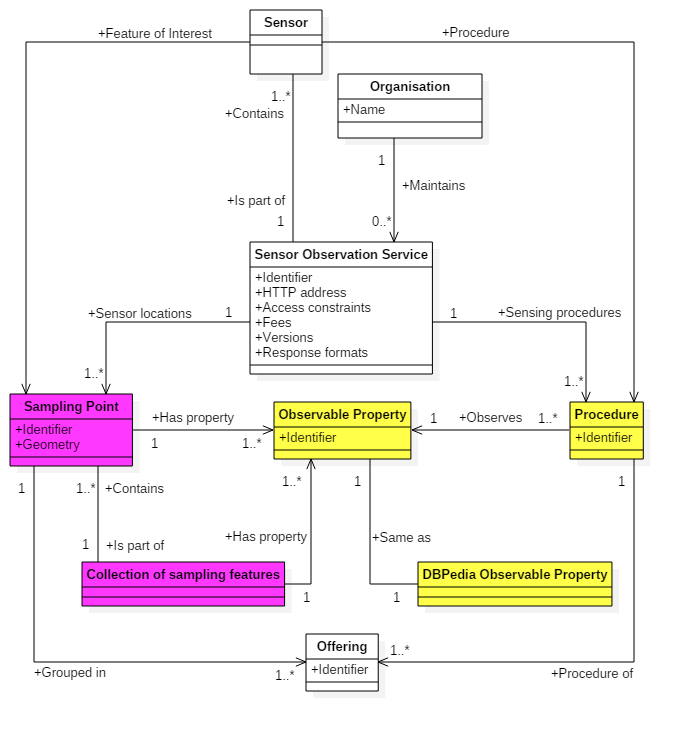
\includegraphics[width=1\linewidth]{UML/SOS_Semantic_UML_2.PNG}
	\caption{Sensor metadata modelled with the om-lite (classes in yellow) and sam-lite (classes in purple) ontologies}
	\label{fig:SOS_Semantic_UML}
\end{figure}

\begin{figure}
	\centering
	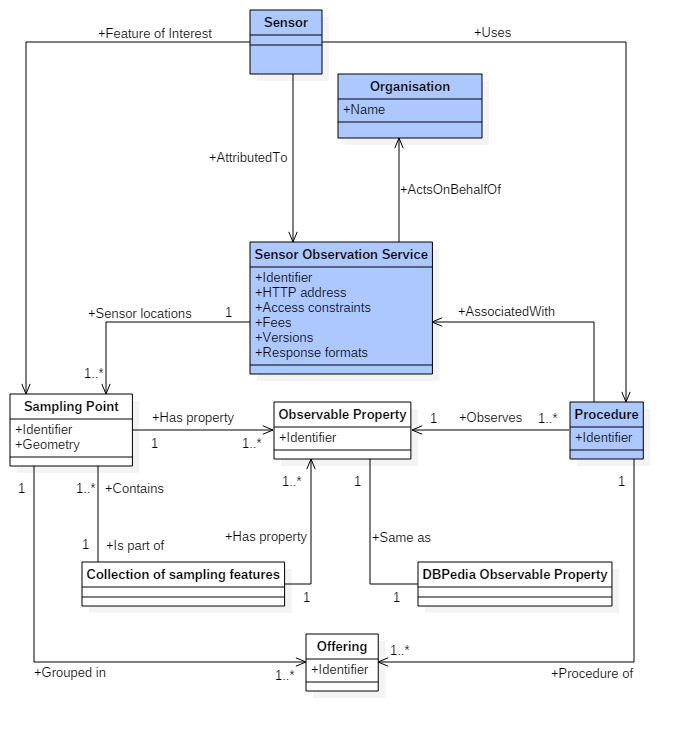
\includegraphics[width=1\linewidth]{UML/SOS_Semantic_UML_3.PNG}
	\caption{Sensor metadata modelled with the PROV ontology (PROV classes in blue)}
	\label{fig:SOS_Semantic_UML2}
\end{figure}

After the metadata has been retrieved from the \ac{sos} and filtered, it has to be mapped to linked data ontologies. For this the om-lite and sam-lite ontologies are being used in combination with the PROV and GeoSPARQL ontologies. Figure \ref{fig:SOS_Semantic_UML} shows how om-lite and sam-lite can be used to describe classes of Figure \ref{fig:SOS_UML}, from an observation perspective. Figure \ref{fig:SOS_Semantic_UML2} shows that classes of Figure \ref{fig:SOS_UML} can be described from a provenance perspective as entities, agents and processes.     

A \ac{sos} is modelled as an agent with a specific name, that acts on behalf of a certain organisation. Every sensor is described by a procedure and a certain feature of interest. The sensor class was not present in the model of Figure \ref{fig:SOS_UML}, because the \ac{sos} does not define sensors. However, the sensor class has been added to the semantic model to make the relation between procedure (type of sensor) and sampling point explicit. 

In Figure \ref{fig:SOS_Semantic_UML} the collection of sampling features is added. These are collections of all \acp{foi} from different \aclp{sos} of which the same property is being observed. The sampling collections are currently modelled to only contain sampling points. This is because the \ac{foi} of an air quality sensor is equal to the bubble of air directly around the sampling location. Other types of sampling features can be added when the application requires this. The offering class is modelled as a specialisation of the collection of sampling features. It contains a subset of the sampling points that are part of the same offering at a particular \ac{sos}.

The last class that has been added to the model as shown in Figure \ref{fig:SOS_Semantic_UML} with respect to the model from Figure \ref{fig:SOS_UML}, is the DBPedia \texttt{observedProperty} class. Every observed property that is defined in a \ac{sos} relates to a certain observed property as defined by DBPedia. Since \ac{sos} requests require their own identifiers as input, the \texttt{observedProperty} class exists twice in the model: one as defined by the \ac{sos} and one as defined by DBPedia. For the same reason all sampling points, processes and offerings have a \texttt{name} attribute in addition to their \ac{uri}. These store the original (non-semantic) \ac{uri}, used by the \ac{sos}. 

\subsection{Modelling with the DBPedia ontology}
Apart from creating a descriptive mapping of classes -- which are used to add semantic meaning to data -- there should also be a mapping of inward links. This creates a bridge between related classes on the semantic web, from which the links trace back to the published semantic sensor metadata. Figure \ref{fig:SOS_DBPedia} shows the mapping between DBPedia classes and \ac{sos} classes. DBPedia contains a very broad description of a \ac{sos}. For discovering specific \aclp{sos} it would be useful if all available \ac{sos} instances are linked to, by this DBPedia definition. For defining class instances the \ac{rdf} schema provides a predicate \texttt{type} which could be used for this purpose. Every procedure or observable property instance represents a real world property or procedure. Some properties and procedures are already available as DBPedia definitions. These definitions should be linked by using the \ac{owl} \texttt{sameAs} predicate. The observable property could also be linked to its corresponding collection of sampling feautures. Since all the features a collection contains share the same observable property, the om-lite predicate \texttt{observedProperty} could be used. More relations could have been added to the model in Figure \ref{fig:SOS_DBPedia}, such as the relation between sensor instances and the DBPedia definition of a sensor. However, links like these are left out, because they would add an overwhelming amount of triples on the side of DBPedia. Furthermore, all sensors can already be traced back via their \acp{foi}, procedures, observed property and \ac{sos}. 
 
 \begin{figure}
 	\centering
 	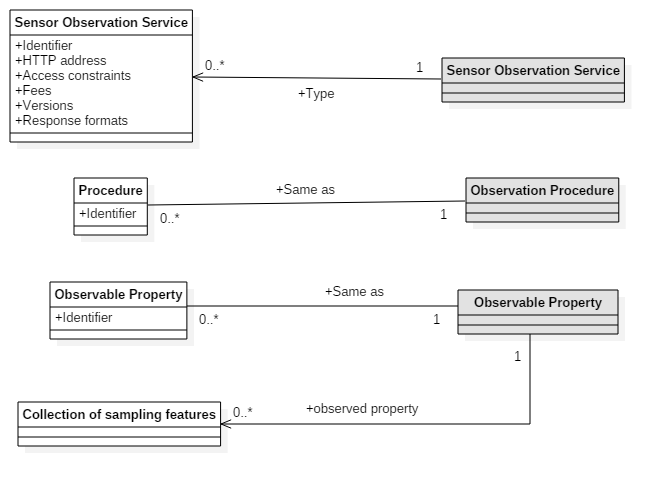
\includegraphics[width=0.9\linewidth]{UML/DBPedia_to_SKB.PNG}
 	\caption{Mapping between DBPedia classes (grey) and SOS classes of Figure \ref{fig:SOS_Semantic_UML} (white)}
 	\label{fig:SOS_DBPedia}
 \end{figure}

\subsection{Output linked sensor metadata}
\label{par:publishLD}

Once the data has been retrieved and mapped to their corresponding classes in the ontologies, \ac{rdf} triples can be created to link the data together. These triples should be stored in files and posted to a \ac{sparql} endpoint. This subsection will describe these steps in more detail.


\subsubsection{Create Resource Description Framework data}
\label{par:createRDF}
For every mapped part of metadata from the \ac{sos}, one or more triples are created. These triples consist of at least \aclp{urn}. However, preferably they are defined by \aclp{url} which can be resolved to an \ac{rdf} document, with semantic information about what it represents. To do so, every part of metadata is automatically assigned a \acf{purl}. For this kind of \ac{url} to resolve, a \ac{purl} server should be set up. Whenever a \ac{purl} is being retrieved, this server performs one of the six tasks shown in Table \ref{tbl:HTTP}. The structure of a \ac{purl} consists of the \ac{http} address of the \ac{purl} server, with a unique identifier attached to it. For example: \url{http://www.examplePURLServer.com/unique\_identifier}. 

Once the metadata is assigned \acp{purl} the triples can be created. Since the metadata of the sensors is being returned by the \ac{sos} in a structured way, links can be created between \acp{url} of \acp{foi}, observable properties, procedures and the other classes shown in Figure \ref{fig:SOS_Semantic_UML} and \ref{fig:SOS_Semantic_UML2}. After these triples have been created the linked data should be serialised to an \ac{rdf} document. The inward links mapping of Figure \ref{fig:SOS_DBPedia} has to be serialised into a separate document. For creating these two documents a notation has to be selected. As described in Section \ref{par:dbpedia} the \ac{rdf} document with DBPedia links should be stored using the N-triples notation. 


\begin{table}[]
	\centering
	\caption{Types of PURLs \citep{LD:PURL}}
	\label{tbl:HTTP}
	\resizebox{\textwidth}{!}{%
		\begin{tabular}{lll}
			PURL Type & Meaning                                         & HTTP Shorthand     \\
			301       & Moved permanently to a target \ac{url}          & Moved Permanently  \\
			302       & Simple redirection to a target \ac{url}         & Found              \\
			303       & See other \acp{url} (use for Semantic Web resources) & See Other     \\
			307       & Temporary redirect to a target \ac{url}         & Temporary Redirect \\
			404       & Temporarily gone                                & Not Found          \\
			410       & Permanently gone                                & Gone              
		\end{tabular}
	}
\end{table}

\subsubsection{Publish RDF on the web}
To store the created linked data a \ac{sparql} endpoint has to be set up. This endpoint is connected to a triple store. The \ac{rdf} documents containing linked data can then be send to the endpoint using \ac{http} POST requests. After it has been stored in the triple store, users can query the triples using the \ac{sparql} query language. 

Once the linked data is inside the triple store, the \acp{purl} can be redirected to \ac{sparql} \texttt{Describe} queries. A \texttt{Describe} query takes a \ac{uri} as input and returns all the triples that contain this \ac{uri} as either subject, predicate or object. This means that all information that the endpoint has about a particular \ac{uri} is being returned. If the \ac{purl} server receives a request for a particular \ac{purl} it makes a \texttt{Describe} query to the endpoint and returns to the client all the linked data that it retrieved about this \ac{purl}.  

The final step in publishing linked data is to make a request to the DBPedia administrators to accept the new links pointing to the observation metadata. This is done by sending a pull request to the DBPedia links GitHub repository, at the following address: \url{https://github.com/dbpedia/links}.


\section{Using logical queries to retrieve sensor data}
\label{par:logicalDesign}
The second web process retrieves a logical query and looks on the semantic web for sensors that observe a certain property in a specific area. It collects the data for these sensors at their corresponding \acl{sos}. When multiple data sources are found, the data is integrated into a single dataset. The sensor data is temporally aggregated before it is returned to the user. Optionally, spatial aggregation can be performed as well.

Figure \ref{fig:WPS2} shows the process of retrieving sensor data. The workflow of this web process is described in Figure \ref{fig:WPS2workflow}.

\begin{figure}
	\centering
	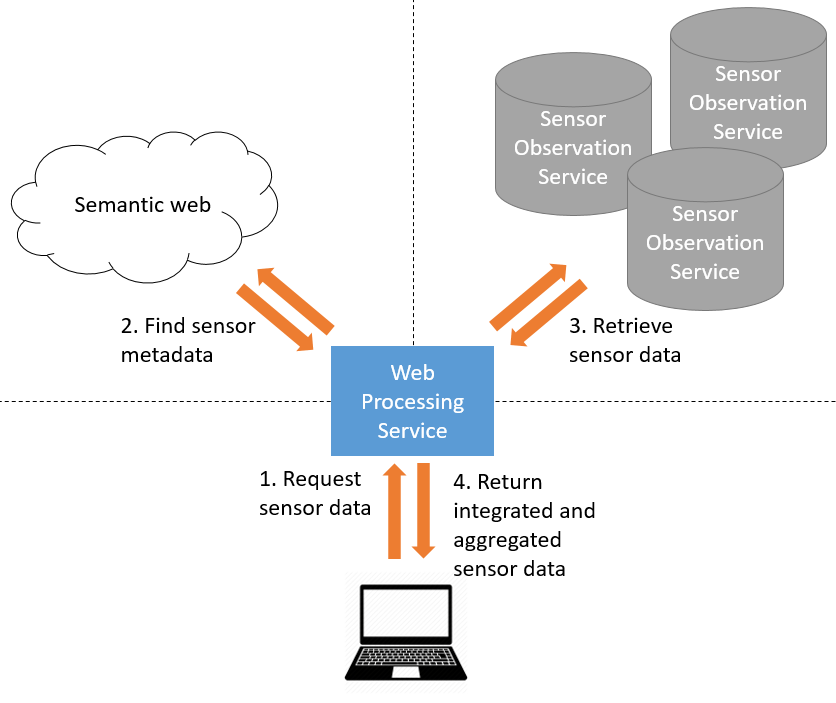
\includegraphics[width=0.8\linewidth]{UML/wps2diagram.PNG}
	\caption{General overview of a Web Processing Service retrieving observation data using linked metadata of Sensor Observation Services}
	\label{fig:WPS2}
\end{figure}

\begin{figure}
	\centering
	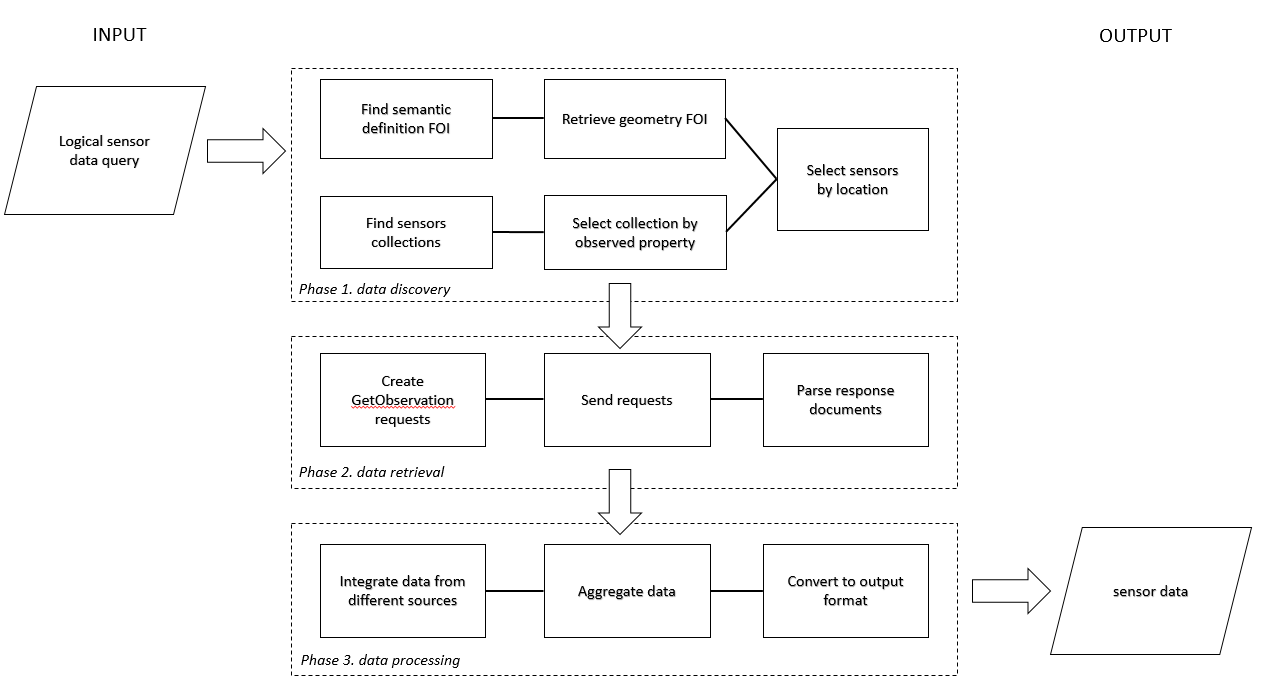
\includegraphics[width=1\linewidth]{UML/wps2workflow.png}
	\caption{Workflow diagram of web process for retrieving sensor data}
	\label{fig:WPS2workflow}
\end{figure}

\subsection{Discovering sensors}
\label{par:discover}
For discovering sensors there are a number of input parameters for the second process: An observed property, a set of names of spatial features, a temporal range and granularity. Additionally, a type of spatial aggregation can be added. The input data, received by the \ac{wps}, is inserted in a number of \ac{sparql} queries. First, the geometry is retrieved for all features inside the input list of \acp{foi}. This is done using the name or identifier attribute of spatial features at the endpoint.  

Then a second \ac{sparql} query selects the sensors that are part of a collection, which observe a certain property of their \acp{foi}. This query also contains a spatial filter with the retrieved geometries, which makes sure only sensors in the requested areas are returned. For all discovered sensors the corresponding \ac{sos} \ac{url}, observed property, offering and process identifiers are retrieved. These original \ac{sos} identifiers are required for creating \texttt{GetObservation} requests.  

\subsection{Retrieving sensor data}
\label{par:retrieve}
 The \ac{sparql} queries return a table with all necessary information per sensor on each row. The columns of this table are: sensor \ac{uri}, \ac{foi} geometry, \ac{foi} identifier, procedure identifier, observed property identifier, offering identifier, and the last column contains the \ac{url} of the \ac{sos}. The data that is returned by the \ac{sparql} queries described in Subsection \ref{par:discover} correspond to the \texttt{GetObservation} input parameters as described in Subsection \ref{par:sos}. This request is send out using all the values per row in the returned table of sensor metadata and is structured by taking the \ac{url} of the \ac{sos} and extending it with: 
 \begin{quote}
 	\url{service=SOS&version=2.0.0&request=GetObservation&procedure=the_procedure&offering=the_offering&observedproperty=the_observed_property&responseformat=http://www.opengis.net/om/2.0&featureOfInterest=the_feature_of_interest}. 
 \end{quote} 
 
 If the \ac{sos} supports temporal filters, they should be added to only retrieve observation data from the temporal range in which the user is interested. To include a temporal filter the following parameters can be added to the above GET request:
\begin{quote}
	\url{&temporalFilter=om:resultTime,start_time/end_time}
\end{quote} 


\subsection{Processing sensor data}
The requests described in Subsection \ref{par:retrieve} result in a \ac{xml} document with observation data for every sensor. In each document the observations have to be retrieved, with their corresponding result time, phenomenon time and \ac{uom}. All of these observation have to be stored in a uniform way in another file or file-like object. If the temporal filter was not supported by the \ac{sos} the observation should only be stored if it is inside the requested temporal range. Also the \ac{foi} geometry should be stored with the observation for data visualisation or spatial aggregation later on. This process repeats itself until the observations have been retrieved from all \ac{xml} documents and they are all stored in a single dataset.  

The next step is to temporally aggregate the observation data. For every sensor location the result time is compared to the temporal range and the value for temporal granularity. Based on the temporal granularity subsets of the temporal range should be selected. After this \textit{temporal sorting} has been performed, all observation values in each of these subsets should be aggregated according to a user defined method. 

If a spatial aggregation method is part of the user's logical query, then it is performed after the temporal aggregation. For each of the spatial features for which observation data has been retrieved, a number of spatially aggregated data is produced. These are the observation results for each time interval (with a length equal to the temporal granularity) inside the temporal range. The spatial aggregation is performed in a similar fashion as the temporal aggregation. First, all observation data are ordered in subset per time interval per spatial feature. After all observations have been ordered the required aggregation method is performed to produce a single value for each of the subsets. 

Examples of aggregation methods that can be used for spatial or temporal aggregation are the average, median, minimum, maximum or sum. Which method is being used is dependent on the kind of information a user needs. Therefore, these methods can be extended with more complex aggregation techniques as described by \cite{SW:Ganesan}. Also, as \cite{SSW:Stasch4} argue semantic reasoning could be implemented to make sure users do not (accidentally) request a meaningless type of aggregation, such as the sum of temperature values over a certain area. 

The last step is to convert the integrated and aggregated data to a desired output format. There are many different formats that could be used for returning sensor data. However, there are two output formats for which an \ac{om} schema has been defined: it can be returned as an \ac{xml} document \citep{SW:ISO} or as a \ac{json} object \citep{SW:OGC6}. The user has the option to retrieve the ouput data in one of these two formats.  



%******************************************************************
%******************************************************************

\chapter{Proof of concept}
\label{chap:impl}
This chapter takes the designed system architecture of Chapter \ref{chap:design} and applies it using existing software tools, and Python libraries and modules to create a proof of concept. First, the data is described which has been used as input for the proof of concept (Section \ref{chap:data}). Following, a detailed description of the implementation of the process for automatically creating linked sensor metadata is provided (Section \ref{par:linkedSD}). After that the implementation of the process for retrieving sensor data using logical queries is shown in Section \ref{par:logicalQuery}. This section starts by showing the web application that has been created as an interface. The fourth part of this chapter describes how the two processes have been made available online in a \acf{wps} (Section \ref{impl:wps}). 

\section{Preparing geographic data}
\label{chap:data}

A number of datasets have been used in this thesis, ranging from observation data inside \aclp{sos} to vector and raster data, which can be used to request data about a certain area or inside certain features. The following subsections will go over the different datasets, describing their sources and contents (Subsection \ref{vector} to Subsection \ref{sensor}). The proof of concept requires the vector and raster datasets as linked data. However, since the spatial features were not available in \ac{rdf}, they had to be converted first. The process of creating linked data of the vector and raster datasets is described (Subsection \ref{linked}).  

\subsection{Vector data}
\label{vector}
For retrieving data inside a spatial feature, vector datasets have been converted to linked data. Data about administrative units are used to allow users to retrieve data about a municipality, province or country. Also, land cover is added to allow user queries to be focused on physical features, such as urban, agricultural or forest areas.   

\subsubsection{Administrative units}
\begin{sloppypar}
	From the Dutch `PDOK' website the datasets of Dutch provinces (\textit{provincies}, Appendix \ref{fig:provinces}) and municipalities (\textit{gemeenten}, Appendix \ref{fig:municipalities}) have been downloaded. This data has been created by the Dutch Cadaster \citep{DATA:Kadaster}. For the Netherlands there are 12 features in the provinces and 393 in the municipalities dataset. 
	
	It was very challenging to obtain data of administrative boundaries of Belgium (even from the \ac{inspire} data portal). Data is offered per municipality, province or region, To create a single  data set of Belgium a large manual effort is required to the different local and regional data sets together. Therefore, all data for Belgium was retrieved from \cite{DATA:GADM}, a website which offers administrative units data sets of almost all countries in the world. This data set of Belgium contains 12 features representing the provinces (including the capitol region of Brussels) and 589 features representing the municipalities.  
	
	The country datasets have also been downloaded from \cite{DATA:GADM} (Appendix \ref{fig:countries}). The administrative unit data has been filtered to contain the names of the administrative units and their corresponding (multi)polygon geometry. 
\end{sloppypar}

\subsubsection{Land cover}
\begin{sloppypar}
	Data on land cover is used to complement the data of administrative units. A section of the 2012 dataset from the \ac{corine} programme, has been selected for this (Figure \ref{fig:CORINE}). The entire CORINE dataset was retrieved from \cite{DATA:CLC}. The features overlapping the Netherlands and Belgium have been retrieved, by performing an intersection operation in the open source QGIS software. The resulting data is stored in a separate database in Postgres. 
	
	The database contains polygon geometries (Appendix \ref{fig:CORINEZOOM}) with a unique identifier and a code that refers to the type of landcover. These codes can be looked up in the accompanied spreadsheet file containing the legend table of \ac{corine} 2012.  	
\end{sloppypar}

\subsection{Raster data}
Data is often used in a raster representation for computations in a \ac{gis}. For natural phenomena a raster representation is especially well suited. The reference grid by \cite{DATA:EEA} is a standard grid which covers Europe. It is available with a resolution of 100km\textsuperscript{2}, 10km\textsuperscript{2} and 1km\textsuperscript{2}. In this thesis the \ac{eea} grid cells with a resolution of 100km\textsuperscript{2} (Appendix \ref{fig:100KM}) and 10km\textsuperscript{2} (Appendix \ref{fig:10KM}) have been used which overlap the Netherlands and Belgium. 15 grid cells of 100km\textsuperscript{2} and 843 grid cells of 10km\textsuperscript{2} have been selected from the original dataset.  

\subsection{Sensor data}
\label{sensor}
\begin{sloppypar}
Air quality sensor data has been used from the \acf{rivm} and from the \acf{ircel}. Both of these organisations have a \ac{sos} where data can be retrieved according to the \ac{swe} standards. The \ac{sos} of the \ac{rivm} (\url{http://inspire.rivm.nl/sos/}) has been online since the 21\textsuperscript{st} of August, 2015. \ac{ircel} has launched theirs on the first of January, 2011 (\url{http://sos.irceline.be/}). Appendix \ref{fig:RIVMSensor} and Appendix \ref{fig:IRCELINESensor} show the sensor networks of both organisations. Their \aclp{sos} provide different kinds of sensor data, such as particulate matter ($PM_{10}$), nitrogen dioxide ($NO_{2}$) and ozone ($O_{3}$). Appendix \ref{fig:Sensor} shows an example of a sensor location in the city centre of Amsterdam. 
\end{sloppypar}

\subsection{Creating linked data of spatial features}
\label{linked}
Linked data has been created in preparation for the proof of concept (Figure \ref{fig:Static}). The data is being used to retrieve and process sensor data on the semantic web. This is done for vector data sets of administrative units and land cover features, and for raster data sets of \ac{eea} grids with a resolution of 10km\textsuperscript{2} and 100km\textsuperscript{2}. The method of \cite{LD:Missier} has been used for this (see Section \ref{par:missier}).

\begin{figure}
	%\centering
	\includegraphics[width=0.7\linewidth]{UML/staticdata2.PNG}
	\caption{Model of vector and raster features}
	\label{fig:Static}
\end{figure}

Three types of administrative units have been converted to linked data: countries, provinces and municipalities. Every administrative unit has a name, type and (multi)polygon geometry assigned to it. The type of administrative units is defined using the DBPedia \ac{uri}s for country, province and municipality. 

The \ac{corine} 2012 land cover dataset contains features with an identifier, a land cover type and a (multi)polygon geometry. The identifier has the form of: \texttt{EU-} plus a unique seven digit number. The land cover type is defined by a three digit number, which can looked up in the provided spreadsheet containing the legend.    

The \ac{eea} reference grid with resolutions of 10km\textsuperscript{2} and 100km\textsuperscript{2}. Every feature is defined by an identifier, a resolution and a point geometry of the origin. The identifier is a code given to a feature by the \ac{eea} and has the form of: resolution + \texttt{E} + x coordinate + \texttt{N} + y coordinate.  


\section{Creating linked data from sensor metadata}
\label{par:linkedSD}

After the linked data of spatial features has been prepared, this chapter continues with creating the proof of concept. The first part of the system architecture described in Chapter \ref{chap:design} is a process which automatically harvests sensor metadata from a \ac{sos} using various requests. The retrieved data should then be mapped to ontologies and serialised to an \ac{rdf} document (Figure \ref{fig:Sequence1}). The next subsections describe how these steps have been implemented using the Python programming language.


\begin{figure}
	\centering
	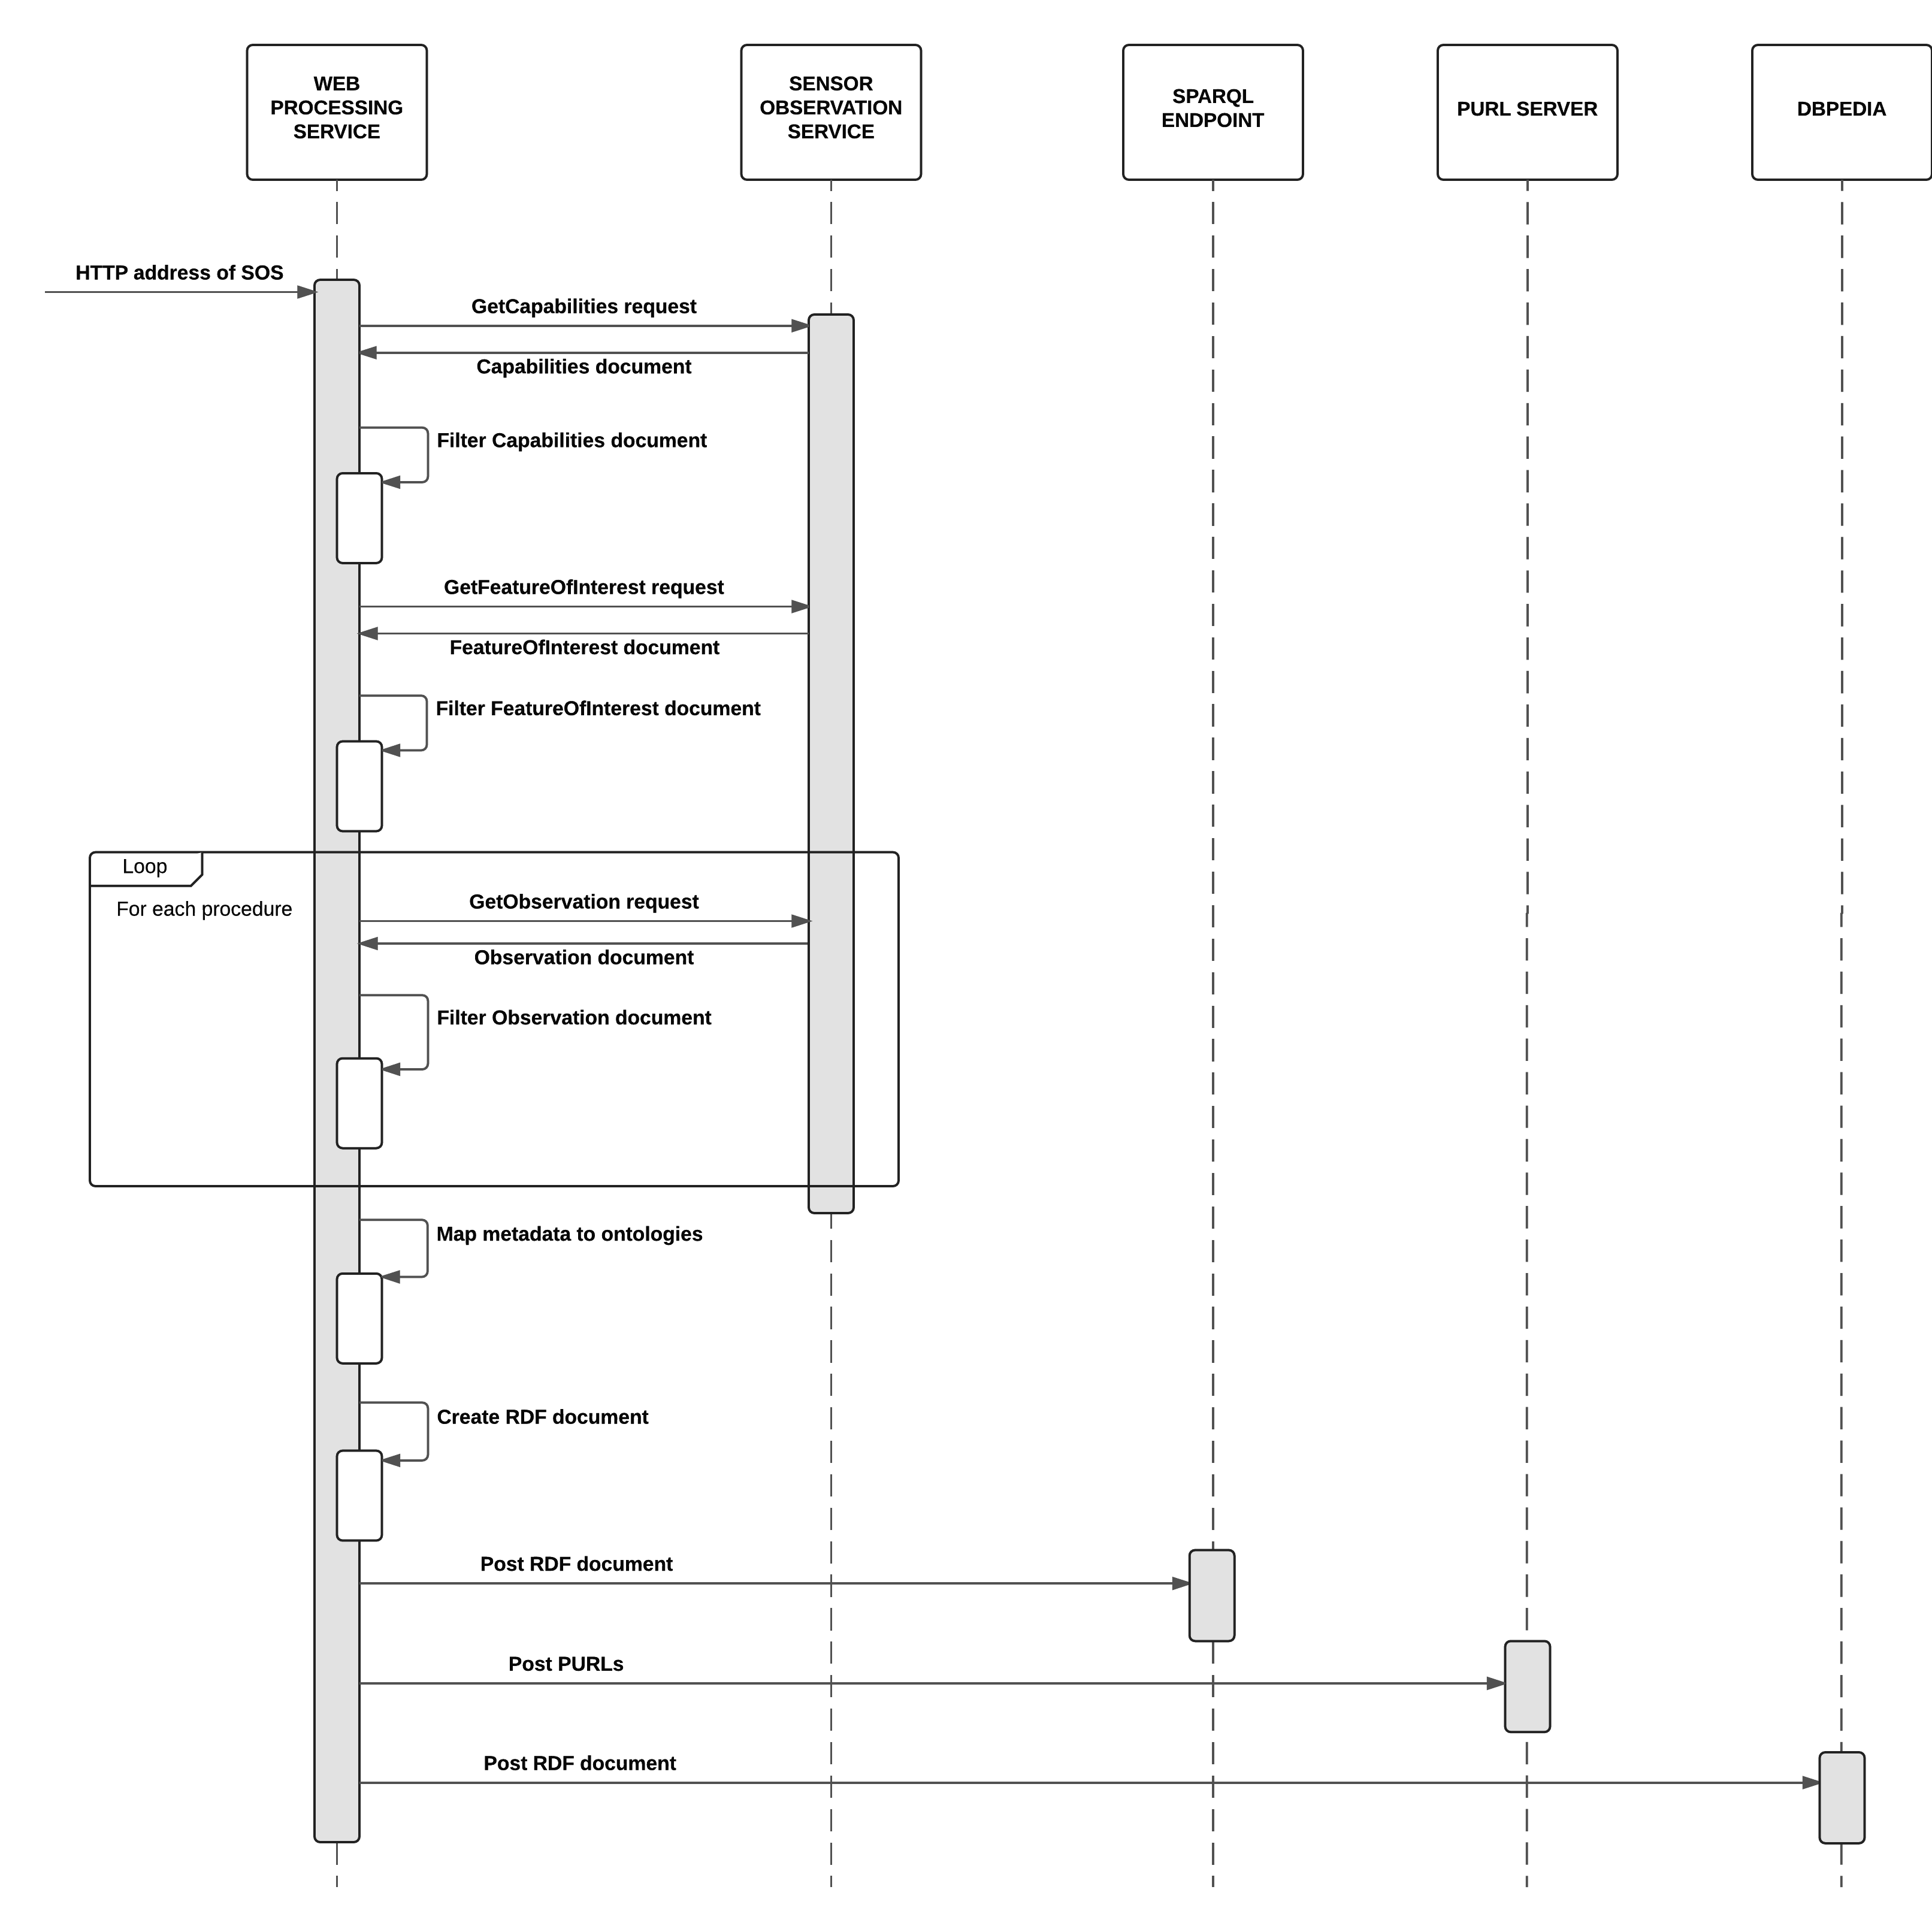
\includegraphics[width=\linewidth]{UML/HarvestSOS.png}
	\caption{UML sequence diagram of the web process for creating linked sensor metadata}
	\label{fig:Sequence1}
\end{figure}

\subsection{Making sensor metadata requests}
A Python class object has been created for the \ac{sos} based on Figure \ref{fig:SOS_UML}. This class contains the different variables and has built in functions to automatically retrieve the metadata. To create a SOSclass instance, the \ac{url} of the \ac{sos} has to be entered as input value. The initialisation of the SOSclass instance creates empty variables for storing information about the \ac{sos}' organisation, supported \ac{sos} versions, response formats, \acp{foi}, offerings, observable properties and procedures. The \acp{foi} are stored in a Python dictionary. This allows information about the \ac{crs}, procedures and observed properties to be added to each \ac{foi}. Similarly, the procedures are stored in a dictionary to be able to easily access which observable property, which \acp{foi} and which offerings are related to a procedure.

\begin{sloppypar}
After the initialisation is finished the method \texttt{SOSclass.request()} is automatically triggered. This function makes all requests to the \ac{sos} shown in Figure \ref{fig:Sequence1}. It starts by sending a \texttt{GetCapabilities} request to the \ac{sos}. For making \ac{http} GET and POST requests the Requests\footnote{\url{http://docs.python-requests.org}} library for Python is used. Code example \ref{lst:Requests} shows how to create a \texttt{GetCapabilities} request with the \ac{http} GET function from this library.
\end{sloppypar}

\begin{sloppypar}
	Based on the content that is being retrieved from the capabilities request further requests are being made. First, the geometries of the \acp{foi} are collected using \texttt{GetFeatureOfInterest} requests. Similar to the \texttt{GetCapabilities} there are no specific parameters required except for: \url{service=SOS&version=2.0.0&request=GetFeatureOfInterest}. However, one of the \aclp{sos} used in this thesis had implemented their \texttt{GetFeatureOfInterest} request to always require a feature id parameter. Therefore, the following exception had to be built, in case this error is returned: \url{service=SOS&version=2.0.0&request=GetFeatureOfInterest&featureOfInterest=allFeatures}.
\end{sloppypar}

\begin{sloppypar}
After the geometries of the \acp{foi} have been retrieved they should be linked to procedures and observable properties. As described in Subsection \ref{par:metadataRequests} it is not mandatory to define these relations in the \texttt{GetCapabilities}, \texttt{GetFeaturesOfInterest} or \texttt{DescribeSensor} response documents. Therefore, small amounts of observation data are requested from the sensors using \texttt{GetObservation} requests.  
\end{sloppypar}

\begin{lstlisting}[float,caption={Creating a HTTP Get request using Python's Request library}, label={lst:Requests}]
import requests

sosURL = "http://example.com/SOS?"

# Create the GetCapabilities request string
GetCapabilities = "{0}service=SOS&request=GetCapabilities".format(sosURL)

# Send the request
r = requests.get(GetCapabilities)

# Print the response document
print r.content

\end{lstlisting}   


\subsection{Map metadata to ontologies}
After each request is send an \ac{xml} document is returned. To retrieve data from these \ac{xml} documents the LXML\footnote{\url{http://lxml.de}} library for Python is used. With this library the \ac{xml} document can be loaded into an Python object, which allows \ac{xml} processing, such as looping through the elements and searching the whole document for elements with specific tags. Code example \ref{lst:LXML} shows a snippet of code that takes the response document retrieved from Code example \ref{lst:Requests} and that uses the LXML library to find all offerings presented in this document. All offerings are returned as a list and stored inside the variable \texttt{SOSclass.offerings}. With this principle, all metadata from the \ac{sos} is retrieved from the \ac{xml} response documents and stored for further processing.    

\begin{lstlisting}[float,caption={Creating an Etree object from an XML response document using Python's LXML library}, label={lst:LXML}]
import lxml

# Store the retrieved document as an Etree object
tree = etree.fromstring(r.content)

# Retrieve the namespaces from the XML document
nsm = tree.nsmap

# Find all subsets of the XML document that are inside a   
# `sos:ObservationOffering' element 
SOSclass.offerings = tree.findall(".//sos:ObservationOffering", nsm)

\end{lstlisting}   
\begin{sloppypar}
Once all the relevant metadata has been retrieved from the \ac{sos} and stored inside the class object, it should be mapped to linked data ontologies (see Figure \ref{fig:Sequence1}). For handling \ac{rdf} the Python package RDFlib\footnote{\url{https://rdflib.readthedocs.org/}} is used.  RDFlib defines an \ac{rdf} graph to which triples can be added. Code example \ref{lst:rdflib} shows a snippet of code that defines an \ac{rdf} graph and adds all procedures of a \ac{sos} to it with the type \texttt{http://def.seegrid.csiro.au/ontology/om/om-lite\#process}. A semantic \ac{url} is defined for each procedure. It is created using a combination of the name of the organisation and a unique number for each procedure. The domain of the \ac{url} points to the \ac{purl} server. The same principle of creating triples from sensor metadata is applied to all classes and relations described in Figure \ref{fig:SOS_Semantic_UML} and \ref{fig:SOS_Semantic_UML2}. 
\end{sloppypar}


\begin{lstlisting}[float,caption={Creating an RDF graph object with the Python package RDFlib}, label={lst:rdflib}]
import rdflib

# The domain of the PURL server
PURLZ = "http://example.com/PURLZ"

# Create the OM-lite namespace 
oml = rdflib.Namespace("http://def.seegrid.csiro.au/ontology/om/om-lite#")

# Initialise a graph object
g = Graph()

for i, procedure in enumerate(SOSclass.procedures):
	# Define a URIs for the procedures
	procedureURI = URIRef("{0}/{1}_PROC_{2}".format(PURLZ, SOSclass.organisation, i))
	
	# Add all procedures to the graph and define them   
	# as om-lite processes
	g.add( ( procedureURI, RDF.type, oml.Process) )

\end{lstlisting}  

\subsection{Publish linked data}

\begin{figure}
	\centering
	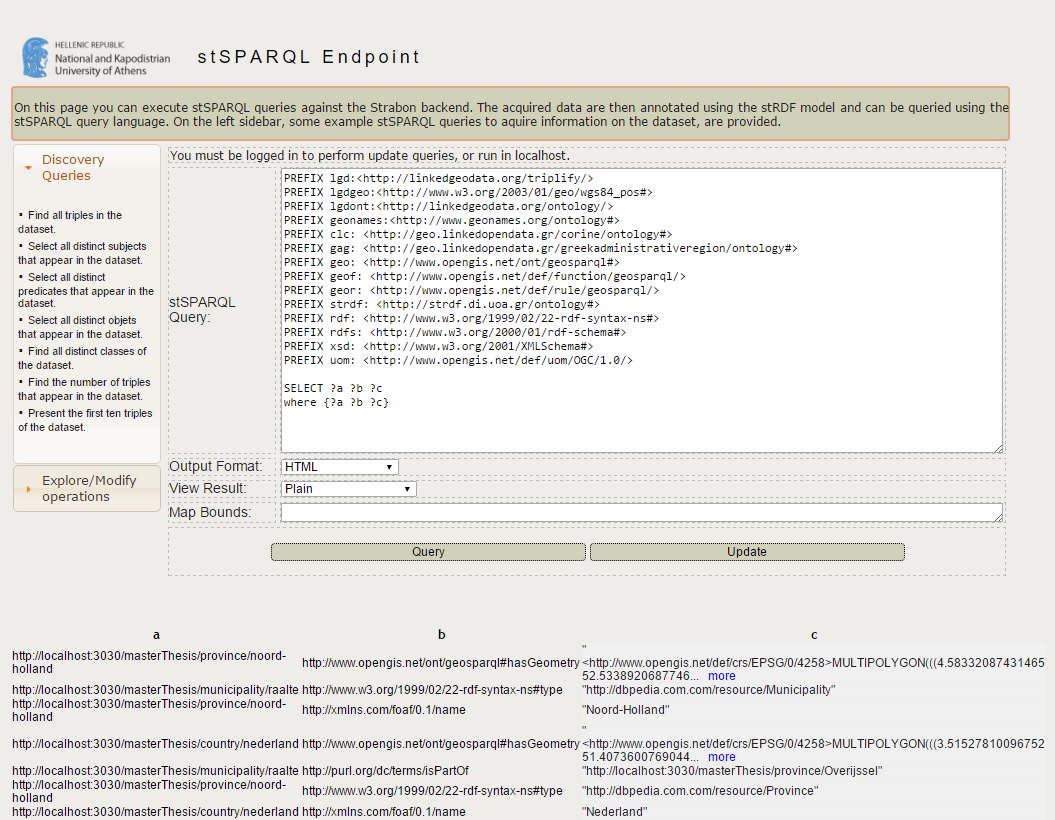
\includegraphics[width=\linewidth]{figs/Strabon.PNG}
	\caption{User interface of the Strabon endpoint}
	\label{fig:Strabon}
\end{figure}

For publishing linked data the Strabon endpoint (Figure \ref{fig:Strabon}) is used in combination with an Apache Tomcat server. The Strabon\footnote{\url{http://strabon.di.uoa.gr/}} endpoint is a semantic spatio-temporal \ac{rdf} store, originally developed for the European  \textit{SemsorGrid4Env} project. It uses a Postgres database with the PostGIS extension to store \ac{rdf} triples. It therefore allows spatial \ac{sparql} queries to be made using the stSPARQL extension (Subsection \ref{par:stSPARQL}).  

The first step of publishing the graph which has been created using RDFlib, is to store it in an \ac{rdf} document. This process is called the \textit{serialisation} of an RDFlib graph. To do this the function \texttt{serialize} of the RDFlib package is used. This function is a method of the graph object and requires two input parameters: the name of the output file and the notation of the triples. In the proof of concept, the Turtle notation is being used. 

After the \ac{rdf} documents have been created they should be posted to the \ac{sparql} endpoint. To post a document to Strabon the client should first login at the endpoint. To do this, a \texttt{Session} object is created using the Requests library. This object posts it login credentials to the endpoint, after which it can be used for posting \ac{rdf} data. Code example \ref{lst:rdflib} shows how to log in to the endpoint with a session object. After that, the graph is serialised to the document \texttt{sensors.ttl}, which can then be posted to the Strabon endpoint.   

\begin{lstlisting}[float,caption={Serializing the RDFlib graph object and posting it to the Strabon endpoint}, label={lst:rdflib2}]
import os
import requests
import rdflib

# Create a new session
session = requests.Session()

# Define the login parameters in a dictionary
login = {"dbname":"endpoint", "username":"your_username", "password":"your_password", "port":"5432", "hostname":"localhost", "dbengine":'postgis"}

# Log in with the session to the Strabon endpoint 
# using the login parameters defined above
r = session.post("http://example.com/strabon-endpoint/DBConnect", data=login)

# Serialize the graph to the file: sensors.ttl
g.serialize("sensors.ttl", format="turtle")

# Post the sensors.ttl file to the endpoint
r = session.post("http://example.com/strabon-endpoint/Store", data={"view":"HTML", "format":"Turtle", "url":"file:///{0}/sensors.ttl".format(os.getcwd()), "fromurl":"Store from URI" }) 
\end{lstlisting}  


For creating \aclp{purl} the Purlz\footnote{\url{http://www.purlz.org/}} software has been used. All \acp{uri} that are created get a \ac{purl} assigned to it. The \ac{purl} resolves the \ac{uri} to a \texttt{DESCRIBE} query at the endpoint. This query is structured as an \ac{http} GET request: \texttt{\seqsplit{http://localhost/strabon-endpoint-3.3.2-SNAPSHOT/Describe?submit=describe\&view=HTML\&handle=download\&format=turtle\&query=DESCRIBE < a\_URI >}}. The request has `\texttt{/Describe?submit=describe}' to call the script that deals with \texttt{DESCRIBE} queries and to tell it that the request is also submitting this type of query. The parameters `\texttt{view=HTML\&handle=download}' indicate that the endpoint's website is requested, but the returned data should be a downloadable file instead of an HTML page. The parameter `\texttt{\&format=turtle}' sets the \ac{rdf} notation of the downloadable file to Turtle and `\texttt{\&query=DESCRIBE <a\_URI>}' is the \ac{sparql} query that contains the \ac{uri} between brackets. 

\begin{lstlisting}[float,caption={Example of a PURL batch file (containing one PURL)}, label={lst:PURL}]
<purls>
	<purl id="/masterThesis_tudelft/responseFormat_0" type="302">
		<maintainers>
		<uid>admin</uid>
		</maintainers>
		<target url="http://example.com/strabon-endpoint/Describe?
			view=HTML&amp;handle=download&amp;
			format=turtle&amp;submit=describe&amp;query=DESCRIBE 
			&lt;http://localhost:8099/masterThesis_tudelft/RIVM_PROC_0&gt;"/>
	</purl>
</purls>
\end{lstlisting}

Every \ac{uri} that is assigned to a part of sensor metadata (like the \texttt{procedureURI} in Code example \ref{lst:rdflib2}) is written to an \ac{xml} file with the parameters: ID, \ac{purl} type, and target address. Optionally, information about the person or organisation maintaining the \ac{purl} can be added. The ID is the original \ac{uri} that is being resolved to the target address. The \ac{purl} type is set to 302, which means that it redirects the client to the target address. Alternative types can be found in Table \ref{tbl:HTTP}. After all \acp{uri} have been added to the so-called \ac{xml} \textit{batch} file as described by \cite{LD:PURL2}, the file can be posted to the Purlz server. Posting \ac{xml} documents to the \ac{purl} server is similar to posting \ac{rdf} documents to the Strabon endpoint as shown in Code example \ref{lst:rdflib2}. An example of a batch file can be seen in Code example \ref{lst:PURL}. These \ac{xml} files are created using the Python package LXML. 

Chapter \ref{chap:design} also describes how to establish inward links from DBPedia, which improve the discovery of sensor metadata. However, this part of the method has not been implemented in the proof of concept, because the proof of concept has been tested locally. The DBPedia knowledge base is available online for a large user audience and can therefore only accept links to reliable resources. Once the method presented in this thesis has been further developed into a stable web process this functionality can be added as well. However, at the moment it could not be part of the proof of concept implementation.  

\section{Using logical queries to retrieve sensor data}
\label{par:logicalQuery}
Section \ref{par:linkedSD} described how the proof of concept implementation harvests sensor metadata from a \ac{sos} and publishes it as linked data in a \ac{sparql} endpoint. The process presented in this section uses that data and its semantics, to automatically retrieve observations based on a user's logical query (Figure \ref{fig:Sequence2}). For handling this process the \texttt{request} class has been created in Python, based on the architecture of Section \ref{par:logicalDesign}. It has been implemented to store all logical input parameters, automatically convert them to \ac{sos} requests using the semantic web and to return the data in an integrated and aggregated way. The next subsection will first introduce the user interface, after which the following subsections describe how the different parts of the process have been implemented.

\begin{figure}
	\centering
	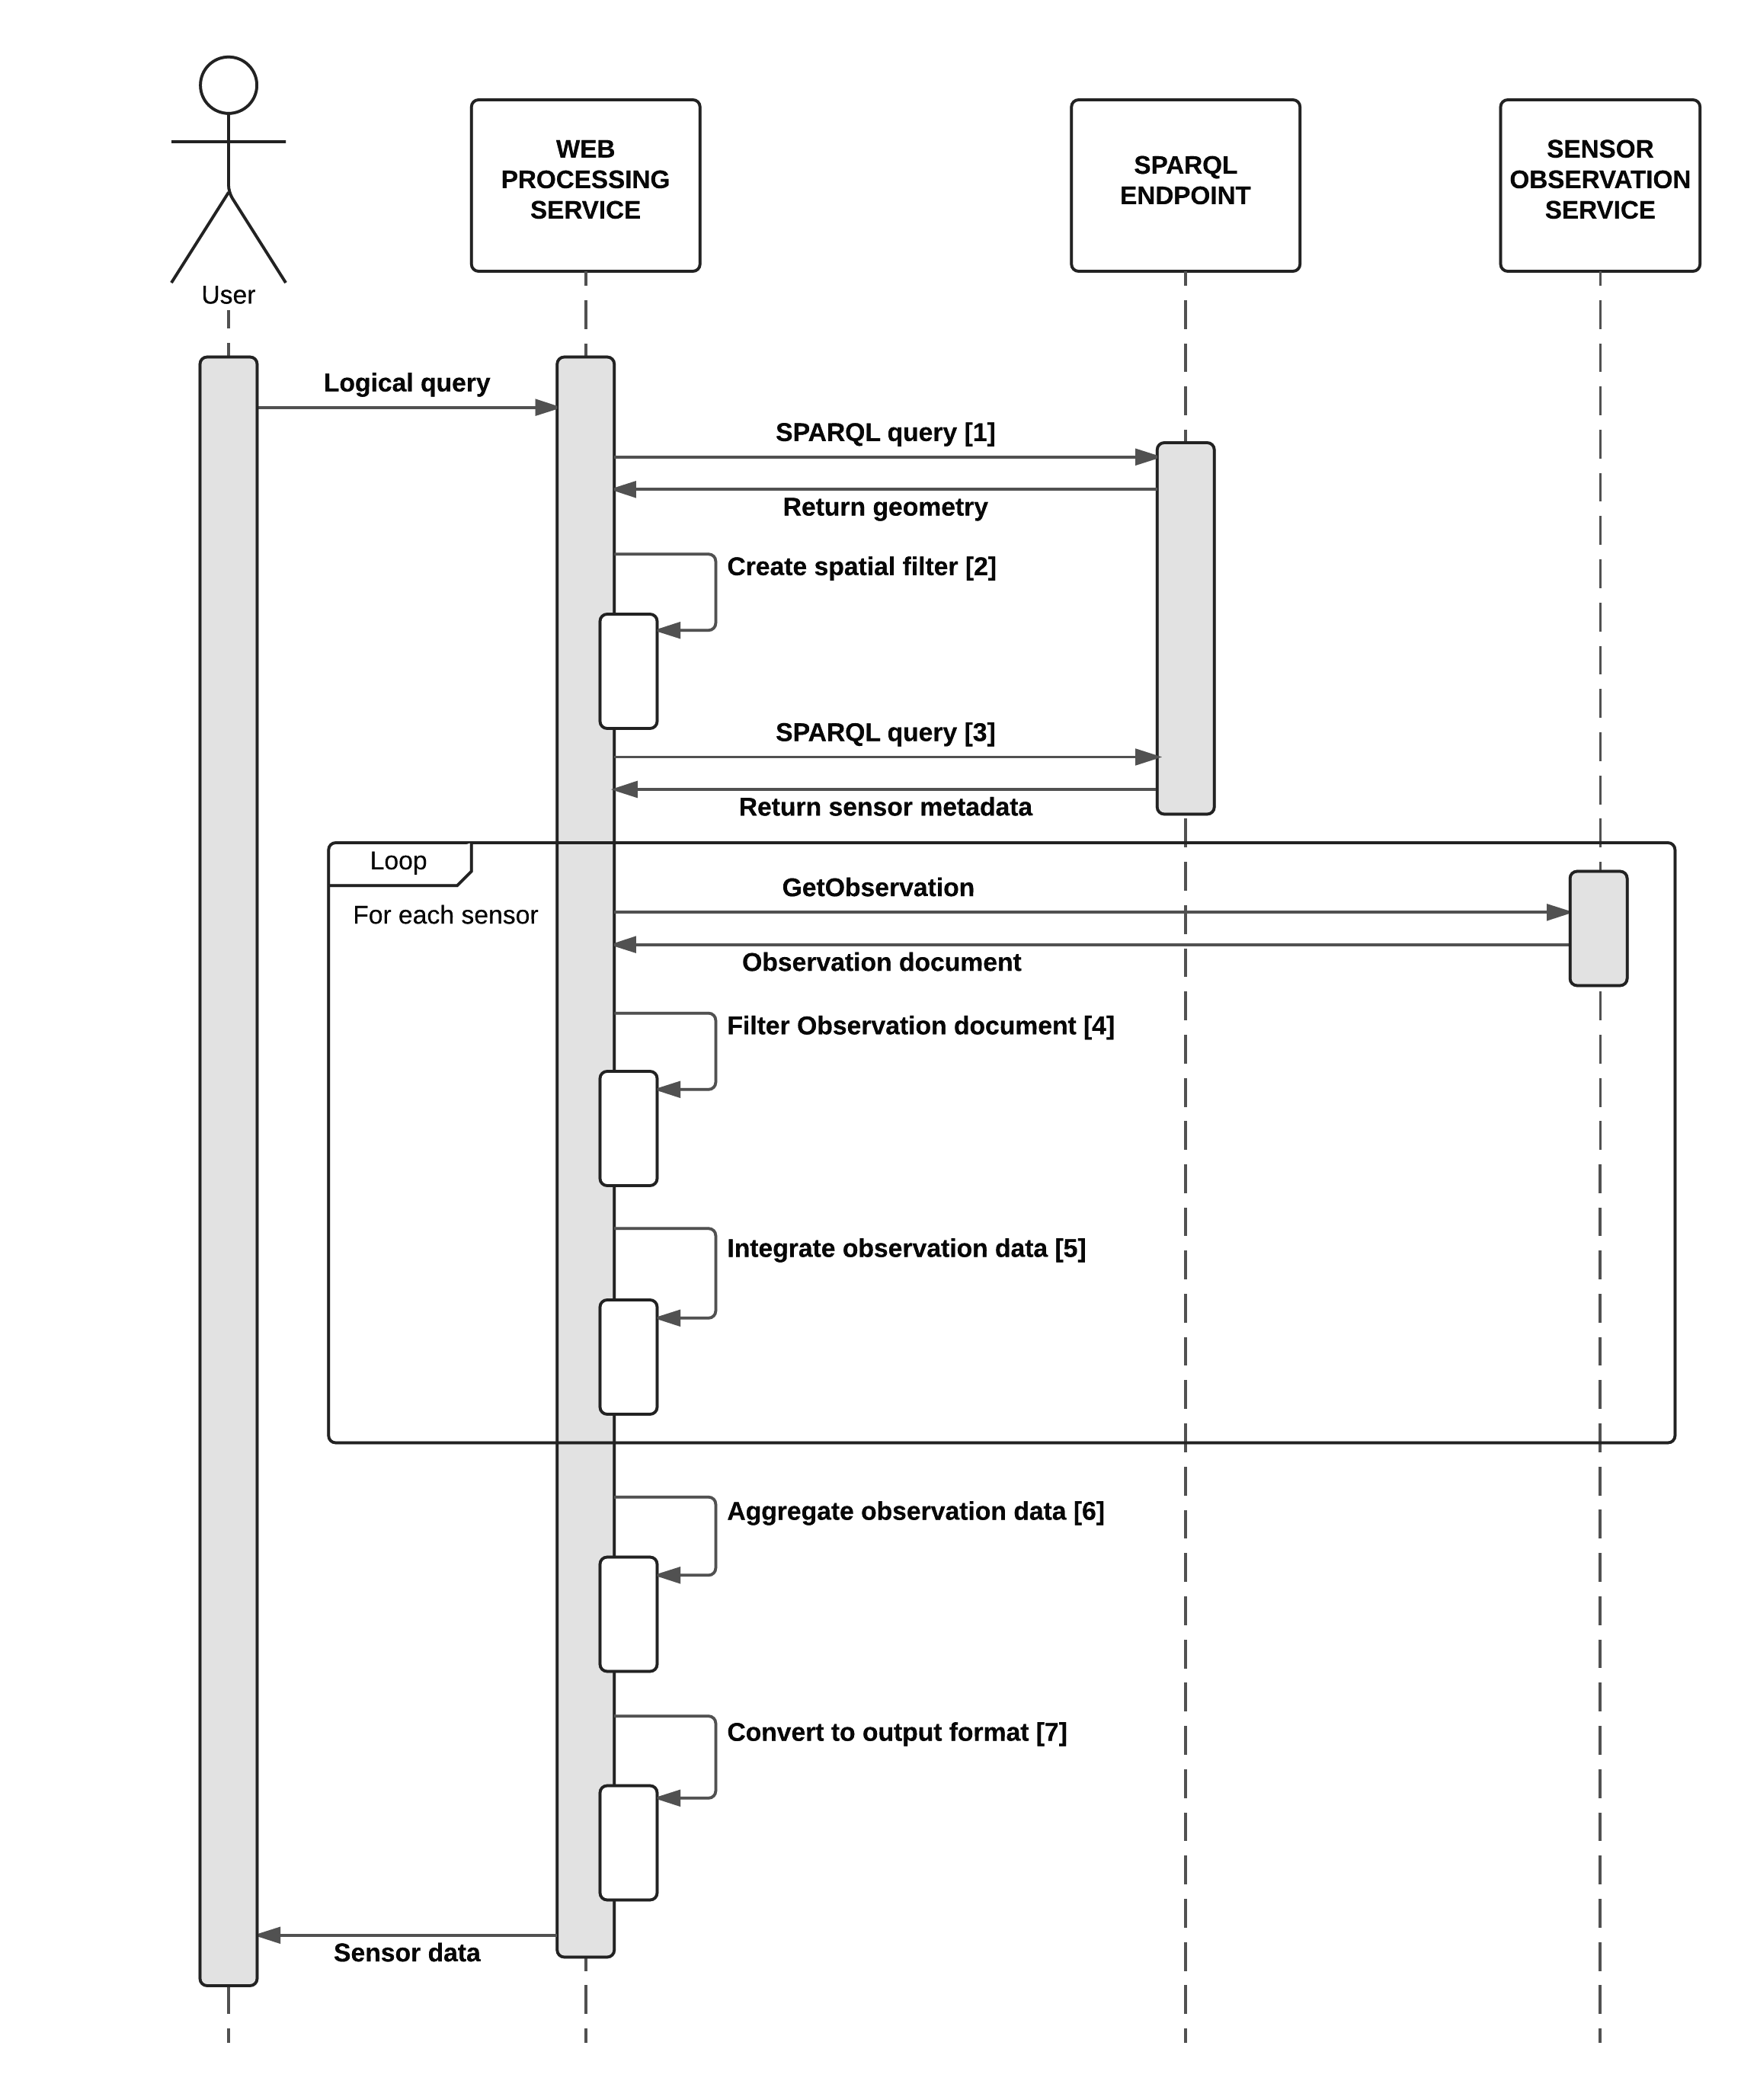
\includegraphics[width=\linewidth]{UML/RetrieveSensorData.png}
	\caption{UML sequence diagram of the web process for retrieving sensor data}
	\label{fig:Sequence2}
\end{figure}

\subsection{Web application for retrieving sensor data}
\label{par:webApp}
The proof of concept implementation takes a number of input parameters. First of all, the observable property, which will be related to a DBPedia definition. The second parameter is the category of input features. This can be set to administrative units (country, province or municipality), land cover or raster. The third parameter is a list of input features. This is a list of names or identifiers that correspond to the category of input features. For example, \textit{Delft municipality} can be used as input since it includes the feature name and its category. The next parameter is the temporal range. This has to be a list of two \ac{iso} datetime strings representing the start and end time. The fifth parameter is the temporal granularity, represented by an integer and a datetime unit, like hour(s), day(s) or week(s). For example, a temporal range of \textit{1 hour} will aggregate the data temporally to a single value per hour. The sixth input parameter is the temporal aggregation method. This is the method for aggregating data between start and end time using the provided temporal granularity. The last input parameter is the method of spatial aggregation. This method will be applied to aggregate observation data per input feature.       

A web application has been created as an interface for the proof-of-concept implementation. It has been created using Flask\footnote{\url{http://flask.pocoo.org/}}, which is a microframework for creating web applications with Python. The first interface that users see is a map on which features can be selected (Figure \ref{fig:interface1}). This can be done by either clicking on them or by manually writing their names in the form below. Also an observed property can be selected in this form.

When the user submits this form the \ac{wps} starts looking for sensors that observe this property and that are located in the selected area (with the \ac{sparql} queries shown in Figure \ref{fig:Sequence2}). Once the sensors have been found they are visualised on the map as orange dots, which can be clicked on to see their \ac{uri}, the observed property \ac{uri} and the \ac{http} address of the corresponding \ac{sos} (Figure \ref{fig:interface2}). Below the map a new form is loaded, which allows users to select spatial and temporal aggregation methods and a temporal range (Figure \ref{fig:interface3}). As the user submits these preferences the \ac{wps} starts retrieving observation data, from the \aclp{sos} that contain the selected sensors. After the process of Figure \ref{fig:Sequence2} has finished, the web application returns a graph to the user, providing a visual impression of the data (Figure \ref{fig:interface4}). The graph is created using Vega-Lite\footnote{\url{https://vega.github.io/vega-lite/}}, a high-level visualisation grammar, developed by Interactive Data Lab of the University of Washington. This graph can be exported as a .PNG image. Alternatively, the data itself can also be downloaded.   

\begin{figure}
	\centering
	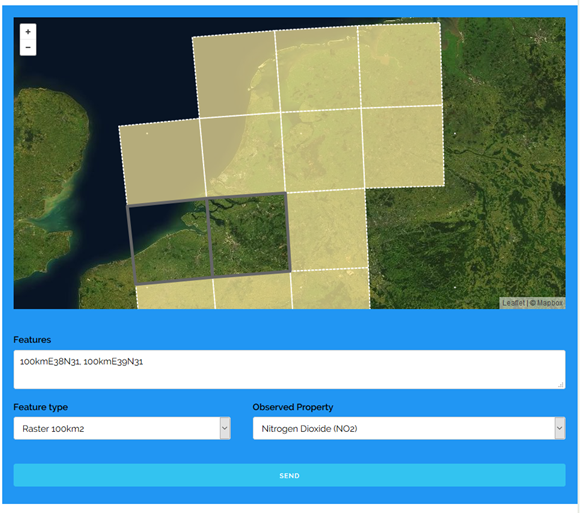
\includegraphics[width=\linewidth]{figs/interface1.PNG}
	\caption{Request sensor data interface (step 1) with parameters for observed property and spatial features}
	\label{fig:interface1}
\end{figure}

\begin{figure}
	\centering
	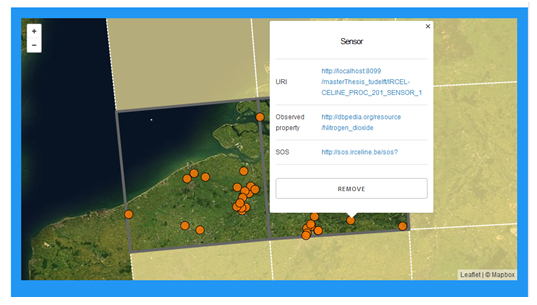
\includegraphics[width=\linewidth]{figs/interface3.PNG}
	\caption{Selecting a sensor on the map shows the semantic \ac{url} of the sensor, its observed property and the address of its \ac{sos}}
	\label{fig:interface2}
\end{figure}

\begin{figure}
	\centering
	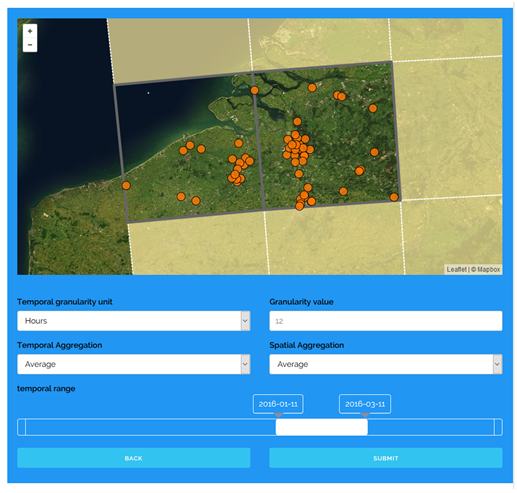
\includegraphics[width=\linewidth]{figs/interface2.PNG}
	\caption{Request sensor data interface (step 2) with parameters for temporal granularity, spatial and temporal aggregation methods and temporal range}
	\label{fig:interface3}
\end{figure}

\begin{figure}
	\centering
	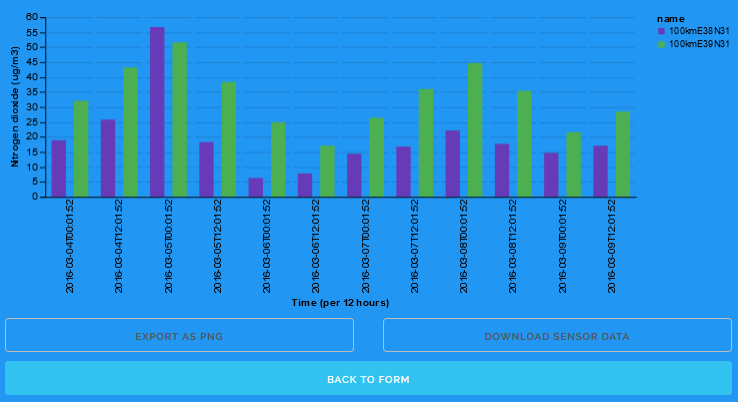
\includegraphics[width=0.9\linewidth]{figs/interface4.PNG}
	\caption{Returned observation data is visualised as a vega-lite graph, with the option to export the graph or download the data}
	\label{fig:interface4}
\end{figure}  


\subsection{Discovering sensors}
\label{par:discoverSensors}
The input category is the starting point for the process to find the geometries of the input features. It creates a \ac{sparql} query that retrieves the geometries of the features by selecting all features of the input category and filtering them by name. Code example \ref{lst:getGeometries} shows that the filter expression is defined first. This expression is added to the a predefined template of a \ac{sparql} query together with the feature category. For the currently implemented categories (landcover, raster, municipalities and provinces) the \ac{url} is found by adding it to DBPedia's standard method for defining \acp{uri}: \url{http://dbpedia.org/resource/}.    

\begin{lstlisting}[float,caption={Example script that sends a SPARQL query for retreiving geometries of input features}, label={lst:getGeometries}]
import requests 

# Define the location of the endpoint
myEndpoint = 'example.com/strabon-endpoint/Query'

for i, feature in enumerate(self.featureNames):
	
	# Create a list with a filter expression for every name 
	featureNamesList = '?name = "{0}"'.format(feature)
	
	# Join them together and place them inside the SPARQL filter function
	featureFilter = "FILTER( {0} )".format( " || ".join(featureNamesList) )


# Define the SPARQL query
query = """
	SELECT 
		?feature ?geom ?name
	WHERE {{ 
		?feature <http://www.w3.org/1999/02/22-rdf-syntax-ns#type> <http://dbpedia.org/resource/{0}> . 
		?feature <http://strdf.di.uoa.gr/ontology#hasGeometry> ?geom . 
		?feature <http://xmlns.com/foaf/0.1/name> ?name . 
	{1}
	}}""".format(self.featureCategory.title(), featureFilter)

# POST the SPARQL query to the endpoint
r = requests.post(myEndpoint, data={'view':'HTML', 'query': query, 'format':'SPARQL/XML', 'handle':'download', 'submit':'Query' }) 

# Print the results
print r.content
\end{lstlisting}

A \ac{sparql} query is then made to find a sensor collection that is related to the requested observed property. From this collection sensors are selected that overlap with the previously found geometries. Unfortunately \ac{sparql} queries are not allowed to exceed a certain number of characters. This creates problems when querying larger vector geometries (provinces and countries). For these queries two alternatives have been implemented as well: using the \ac{eea} reference grid as a spatial index for vector geometries and using bounding box queries at the \ac{sos}. 

For the first alternative the \ac{eea} raster cells are retrieved instead of the vector data. Only the cells are requested that overlap with the vector geometry. For these cells all sensor locations are requested. However, the result of this is that too many sensor locations are retrieved, also some that are outside the original vector feature. Therefore, the \ac{wps} performs the spatial filter afterwards and removes all locations that are outside of the requested feature. 

This type of query is shown in Code example \ref{lst:getSensors}. The raster cells are added in the spatial filter expression and a DBPedia \ac{uri} of an observed property is added instead of the \texttt{<<insert\_observed\_Property>>} placeholder. Multiple spatial features can be put in the filter expression using the logical OR operator. With these two parameters, the query can find all relevant sensors from different sources stored at the endpoint using the model shown in Figure \ref{fig:SOS_Semantic_UML}. It also returns all necessary data to make \texttt{GetObservation} requests at the sensors' corresponding \aclp{sos}.

The second alternative checks which \aclp{sos} have sensors observing a certain property, within the bounding box of the requested vector geometry. The response of the \ac{sparql} query is a set of \aclp{sos}. For all of these services \texttt{GetObservation} requests are made containing a spatial filter. This performs the detailed spatial querying on the \ac{sos} side, instead of at the endpoint. 

\begin{lstlisting}[float,caption={A spatial SPARQL query for discovering sensors and their SOS related metadata}, label={lst:getSensors}]

PREFIX rdf: <http://www.w3.org/1999/02/22-rdf-syntax-ns#>
PREFIX strdf: <http://strdf.di.uoa.gr/ontology#>
PREFIX oml: <http://def.seegrid.csiro.au/ontology/om/om-lite#>
PREFIX saml: <http://def.seegrid.csiro.au/ontology/om/sam-lite#>
PREFIX foaf: <http://xmlns.com/foaf/0.1/>
PREFIX owl: <http://www.w3.org/2002/07/owl#>
PREFIX dbp: <http://dbpedia.org/resource/>
PREFIX dc: <http://purl.org/dc/terms/>

SELECT 
	?sensor ?geom ?FOIname ?procName ?obsPropertyName ?offeringName 
	?sosAddress
WHERE {
	?collection rdf:type saml:SamplingCollection .
	?collection omlite:observedProperty <<insert_observed_Property>> .
	<<insert_observed_Property>> owl:sameAs ?obsProperty .
	?obsProperty foaf:name ?obsPropertyName .
	?collection saml:#member ?FOI .
	
	?offering saml:member ?FOI . 
	?offering prov:specializationOf ?collection .
	?offering foaf:name ?offeringName .
	
	?FOI strdf:hasGeometry ?geom . 
	?FOI foaf:name ?FOIname  .
	
	?sensor oml:featureOfInterest ?FOI .
	?sensor oml:procedure ?procedure .
	?sensor dc:isPartOf ?sos .
	?sos owl:sameAs ?sosAddress .
	
	?procedure omlite:observedProperty ?obsProperty .
	?procedure foaf:name ?procName .
	?offering oml:procedure ?procName .
	
	FILTER(
		strdf:contains("POLGYON(( <<insert_coordinates>> ))"^^strdf:#WKT, ?geom)
	)		
}
\end{lstlisting}

\subsection{Retrieving sensor data}
\begin{sloppypar}
After all sensor locations have been retrieved from the \ac{sparql} endpoint \texttt{GetObservation} requests are made. These require the identifiers of observed properties and procedures which were given by their \ac{sos}, instead of the semantic \acp{url} which were assigned to them later. The requests are structured as explained in Subsection \ref{par:getObservation}. When possible, the request is extended with a temporal filter to only retrieve data inside the required temporal range. The output format is set to \ac{xml} using the \url{http://www.opengis.net/om/} schema.
\end{sloppypar}

Code example \ref{lst:getObservation} shows how to use the LXML Python package to create a spatial filter in \ac{xml} which can be added to a \texttt{GetObservation} POST request. For all retrieved sensor data using this approach, the client still has to check whether the returned \acp{foi} are really inside the vector geometry requested by the user. 

\begin{lstlisting}[float,caption={Script that creates an LXML graph object called spatialFilter to add to a \texttt{GetObservaton} POST request}, label={lst:getObservation}]
spatialFilter = etree.SubElement(getObservation, "{http://www.opengis.net/sos/2.0}spatialFilter")

bbox = etree.SubElement(spatialFilter, "{http://www.opengis.net/fes/2.0}BBOX" )

valueReference = etree.SubElement(bbox, "{http://www.opengis.net/fes/2.0}ValueReference")
valueReference.text = "om:featureOfInterest/sams:SF_SpatialSamplingFeature/sams:shape"

envelope = etree.SubElement(bbox, "{http://www.opengis.net/gml/3.2}Envelope")
envelope.attrib["srsName"] = "http://www.opengis.net/def/crs/EPSG/0/4258"

LLcorner = etree.SubElement(envelope, "{http://www.opengis.net/gml/3.2}lowerCorner")
LLcorner.text = "{1} {0}".format(Xmin, Ymin)
URcorner = etree.SubElement(envelope, "{http://www.opengis.net/gml/3.2}upperCorner")
URcorner.text = "{1} {0}".format(Xmax, Ymax)
\end{lstlisting}

\begin{sloppypar}
The \ac{xml} documents received from the \texttt{GetObservation} requests, are loaded into Python using the LXML package. The first step is to find all \texttt{sos:observationData} elements inside it. These elements contain observations according to the \ac{om} schema. There are however, some implementation differences in the response documents. Some \aclp{sos} return sensor data as an \ac{om} measurement. Others use the \texttt{swe:dataArray} type. A response document with the \ac{om} measurements contains separately nested elements for each individual observation. Every observation result has its own element defining the result value, result time, \ac{uom}, procedure, \ac{foi} and observed property.  
\end{sloppypar}

The \ac{swe} data array is an array of observations that share the same metadata. For all observations which have the same feature of interest, procedure, observed property and \ac{uom}, the result data is joined together into an array of result values combined with the result or phenomenon time. The result value is separated from the result or phenomenon time using a predefined \textit{tokenseparator}. Each individual observation in the data array is separated using a predefined \textit{blockseparator}. The data from the received \ac{xml} documents is directly added to an individual comma separated value string per combination of observed property and \ac{uom}. When the temporal filter cannot be used, all data is looped over first, to remove observations outside the temporal range. 

\subsection{Data aggregation}
After all observation data is retrieved, it is first aggregated temporally. An empty dictionary is created to store each temporal granularity range, which is inside the requested temporal range for all observations. A loop goes over the comma separated values and sorts them based on their result time per sensor location. The start time is subtracted from the result time, which outputs the time range from the start of the temporal range to the time of the observation. From this time range a modulo operation calculates the ratio between the temporal granularity and the time range between the start of the temporal range and the time of the observation. A dictionary key is created to sort the observations. To calculate the key the temporal granularity is multiplied by the outcome of the modulo operation, after which the start time is added to it. 

As soon as all the observations have been sorted the data is aggregated. For all values per key the average, minimum, maximum, median or sum is calculated. The resulting value replaces the values in the dictionary. Code example \ref{lst:aggregate} shows how the observation data stored as strings containing comma separated values, can be quickly aggregated to a single value. If spatial aggregation is part of the sensor data request, this is performed after the temporal aggregation. Using Shapely's 9-intersection model functions, the sensor locations are ordered per spatial feature. Finally, all values are aggregated for each feature per temporal range. For both temporal and spatial aggregation the basic methods have been implemented such as average, minimum, maximum, sum and median. These methods can be further extended to give more reliable results \citep{SW:Ganesan} or to give more semantic meaning to the aggregation methods \citep{SSW:Stasch4}.         


\begin{lstlisting}[float,caption={Script that performs basic temporal aggregation methods on a comma separated value string}, label={lst:aggregate}]
import numpy

# Example comma separated value string 
csvString = "2016-06-25T09:00:00,15.2;2016-06-25T09:02:00,15.5"

# split the string into a list with individual 
# observations using the block separator 
observations = csvString.split(";")

# Aggregate the observations with a method selected by the user
if self.tempAggregation == "average":
	aggregatedData = (sum([float(x.split(",")[1]) for x in observations]) ) / float(len(observations))
elif self.tempAggregation == "minimum":
	aggregatedData = min([float(x.split(",")[1]) for x in observations])
elif self.tempAggregation == "maximum":
	aggregatedData = max([float(x.split(",")[1]) for x in observations])
elif self.tempAggregation == "sum":
	aggregatedData = sum([float(x.split(",")[1]) for x in observations])
elif self.tempAggregation == "median":
	aggregatedData = numpy.median(numpy.array([float(x.split(",")[1]) for x in observations]))
\end{lstlisting}


\begin{lstlisting}[float,caption={Script that defines a web proces using PyWPS}, label={lst:PyWPS}]
from pywps.Process import WPSProcess
from sosRequests import *
from linkedDataCapabilities import *

class Process(WPSProcess):

	def __init__(self):

		WPSProcess.__init__(self,
			identifier = "LinkedDataFromSOS",
			title="Creates Linked Data of SOS metadata",
			abstract="""This process takes an HTTP address of a Sensor Observation Service (SOS) as input 	and converts the metadata to linked data.""",
			version = "1.0",
			storeSupported = True,
			statusSupported = True)

		# Adding process input
		self.urlIn = self.addLiteralInput(
			identifier = "input_url", 
			title = "Input a string containing an HTTP address of a Sensor Observation Service (SOS). For example: 'http://someaddress.com/sos?'", 
			default = "http://inspire.rivm.nl/sos/eaq/service?", 
			type = "StringType")

		def execute(self):
			url = self.urlIn.getValue()

			# Create SOS instance with the URL as input and 
			# retrieve its metadata.  
			sos = SOS(url)

			# Create and publish linked data from the above 
			# retrieved metadata
			linkedDataCapabilities(sos)

if (__name__ == "__main__"):
	Process = Process()
	Process.execute()
\end{lstlisting}

\section{Setting up the Web Processing Services}
\label{impl:wps}

The proof of concept web processes described in Section \ref{par:linkedSD} and \ref{par:logicalQuery} have been added to a \ac{wps} using the PyWPS software. PyWPS is an implementation of the \acl{wps} standard from the \acl{ogc} using the Python programming language. It is an open source project and aims to enable the integration, publishing and execution of Python processes via the \ac{wps} standard (see \url{http://pywps.org/}).  

Code example \ref{lst:PyWPS} shows how a \ac{wps} process is defined. A PyWPS process is created using the \texttt{Process} class. Instances of this class contain all the functionality and metadata of the \ac{wps} processes. The Process class consists of two parts: the \texttt{\_\_init\_\_} method and the \texttt{execute} method. The \texttt{\_\_init\_\_} method initializes a \ac{wps} process by giving it an identifier, title, abstract, version number, together with other kinds of (optional) metadata. It also defines the inputs and outputs. The \texttt{execute} method is where the functionality of the process is defined. The process in Code example \ref{lst:PyWPS} imports a class called `SOS' with methods for retrieving metadata from a \acl{sos} and a function called `linkedDataCapabilities' to convert this data to \ac{rdf}.

PyWPS has been installed with the method described by \cite{wps:Deltares}. The \ac{wps} is hosted using the XAMPP software. XAMPP is an open source Apache distribution, that includes a number of useful features such as the Tomcat server (used for hosting of the Strabon endpoint). A \texttt{pywps.cgi} file is defined, which points to the location of the PyWPS installation and placed in Apache's \textit{cgi-bin} folder. The last step in hosting processes -- such as in Code example \ref{lst:PyWPS} -- is to store the process definition in the \textit{pywps\_processes} folder of the PyWPS installation and adding its identifier to the \texttt{\_\_init\_\_} file in that same folder.    


